\section{HTML \& JavaScript}

\frame{ \tableofcontents[currentsection] }


\begin{frame}
  \frametitle{HTML}
  \begin{center}
    \begin{tikzpicture}[remember picture]
      \path[use as bounding box] (-2.5,-4) rectangle (8,3);

      \node[draw,rectangle split,rectangle split parts=2,inner sep=1mm,anchor=north] (html) at (3,3) {
        {\sc example.html}
        \nodepart{second}
        \inlinecode[language=HTML,font size=\tiny,width=.75\linewidth,frame=none]{example.html}
      };
      \node[draw,anchor=south west,inner sep=1mm,fill=white,rectangle split,rectangle split parts=2] at (-2.5,-4) {
        {\sc resultaat}
        \nodepart{second}
        
\includegraphics[width=4.5cm]{raw-html.png}
      };
    \end{tikzpicture}
  \end{center}
\end{frame}

\begin{frame}
  \frametitle{HTML+CSS}
  \begin{center}
    \begin{tikzpicture}[remember picture]
      \path[use as bounding box] (-2.5,-4) rectangle (8,3);

      \node[draw,rectangle split,rectangle split parts=2,inner sep=1mm,anchor=north] (html) at (3,3) {
        {\sc example.html}
        \nodepart{second}
        \inlinecode[language=HTML,font size=\tiny,width=.75\linewidth,frame=none]{example2-tex.html}
      };
      \node[draw,fill=white,rectangle split,rectangle split parts=2,anchor=north west,inner sep=1mm] (css) at ($ (html.north west) + (4,-2) $) {
        {\sc example.css}
        \nodepart{second}
        \inlinecode[language=CSS,font size=\tiny,width=.4\linewidth,frame=none]{example.css}
      };
      \draw[->,thick] (csslink.east) to[bend left=30] (css.north);
      \node[draw,anchor=south west,inner sep=1mm,fill=white,rectangle split,rectangle split parts=2] at (-2.5,-4) {
        {\sc resultaat}
        \nodepart{second}
        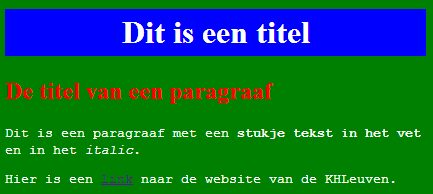
\includegraphics[width=4.5cm]{html-css.png}
      };
    \end{tikzpicture}
  \end{center}
\end{frame}

\begin{frame}
  \frametitle{HTML+CSS+JavaScript}
  \begin{center}
    \begin{tikzpicture}[remember picture]
      \path[use as bounding box] (-2.5,-4) rectangle (8,3);

      \node[draw,rectangle split,rectangle split parts=2,inner sep=1mm,anchor=north] (html) at (3,3) {
        {\sc example.html}
        \nodepart{second}
        \inlinecode[language=HTML,font size=\tiny,width=.75\linewidth,frame=none]{example3-tex.html}
      };

      \node[draw,fill=white,rectangle split,rectangle split parts=2,anchor=north west,inner sep=1mm] (css) at ($ (html.north west) + (4,-2) $) {
        {\sc example.css}
        \nodepart{second}
        \inlinecode[language=CSS,font size=\tiny,width=.4\linewidth,frame=none]{example.css}
      };
      \draw[->,thick] (csslink.east) to[bend left=30] (css.north);

      \node[draw,fill=white,rectangle split,rectangle split parts=2,anchor=north west,inner sep=1mm] (js) at ($ (css.north west) + (1,-2) $) {
        {\sc example.js}
        \nodepart{second}
        \inlinecode[language=javascript,font size=\tiny,width=.4\linewidth,frame=none]{example.js}
      };
      \draw[->,thick] (jslink.south) to[bend right=30] (js.west);

      \node[draw,anchor=south west,inner sep=1mm,fill=white,rectangle split,rectangle split parts=2] at (-2.5,-4) {
        {\sc resultaat}
        \nodepart{second}
        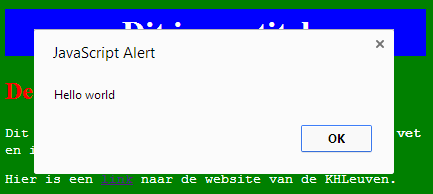
\includegraphics[width=4.5cm]{html-css-js.png}
      };
    \end{tikzpicture}
  \end{center}
\end{frame}

\begin{frame}
  \frametitle{Sjabloon}
  \begin{center}
    \begin{tikzpicture}
      \node[draw,rectangle split,rectangle split parts=2,inner sep=1mm,anchor=north] (html) {
        {\sc html}
        \nodepart{second}
        \inlinecode[language=HTML,font size=\tiny,width=.75\linewidth,frame=none]{template.html}
      };

      \node[draw,rectangle split,rectangle split parts=2,inner sep=1mm,anchor=north] (javascript) at ($ (html.south) + (0,-.5) $)  {
        {\sc code.js}
        \nodepart{second}
        \inlinecode[language=HTML,font size=\tiny,width=.75\linewidth,frame=none]{template.js}
      };
    \end{tikzpicture}
  \end{center}
\end{frame}

\begin{frame}
  \frametitle{Voorbeeld}
  \begin{center}
    \begin{tikzpicture}
      \node[draw,rectangle split,rectangle split parts=2,inner sep=1mm,anchor=north] (html) {
        {\sc html}
        \nodepart{second}
        \inlinecode[language=HTML,font size=\tiny,width=.75\linewidth,frame=none]{template.html}
      };

      \node[draw,rectangle split,rectangle split parts=2,inner sep=1mm,anchor=north] (javascript) at ($ (html.south) + (0,-.5) $)  {
        {\sc code.js}
        \nodepart{second}
        \inlinecode[language=javascript,font size=\tiny,width=.75\linewidth,frame=none]{code.js}
      };

      \node[anchor=north east,inner sep=1mm,fill=white] at (-.5,-5) {
        
\includegraphics[width=4cm]{input.png}
      };
      \node[anchor=north west,inner sep=1mm,fill=white] at (.5,-5) {
        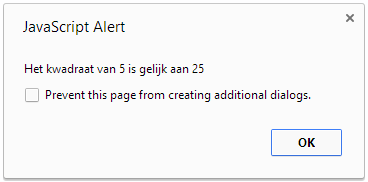
\includegraphics[width=4cm]{output.png}
      };
    \end{tikzpicture}
  \end{center}
\end{frame}


%%% Local Variables: 
%%% mode: latex
%%% TeX-master: "intro"
%%% End: 
